\documentclass[a4paper,11pt]{article}

% ******************************************************************************
% * PACKAGES
% ******************************************************************************

% *** FONT PAcKAGES ***
%\usepackage{times}

\usepackage{psfrag}


% *** MATH PACKAGES ***
\usepackage{amsthm}
\usepackage{amsmath}
\usepackage{amssymb}

% *** CITATION PACKAGES ***
\usepackage{cite}

% *** GRAPHICS RELATED PACKAGES ***
\usepackage[dvips]{graphicx}
\graphicspath{{./Pictures/}}
\DeclareGraphicsExtensions{.eps,.pdf,.png,.jpg}

% *** SPECIALIZED LIST PACKAGES ***
%\usepackage{algorithmic}

% *** ALIGNMENT PACKAGES ***
%\usepackage{array}

%\usepackage{mdwmath}
%\usepackage{mdwtab}

%\usepackage{eqparbox}

% *** SUBFIGURE PACKAGES ***
%\usepackage[tight,footnotesize]{subfigure}

%\usepackage[caption=false]{caption}
%\usepackage[font=footnotesize]{subfig}

% *** FLOAT PACKAGES ***
%\usepackage{fixltx2e}
%\usepackage{stfloats}

% *** PDF, URL AND HYPERLINK PACKAGES ***
%\usepackage{url}
% Usage: \url{my_url_here}.

% correct bad hyphenation here
%\hyphenation{op-tical net-works semi-conduc-tor}


% ******************************************************************************
% * DOCUMENT
% ******************************************************************************

\begin{document}
%
% paper title
% can use linebreaks \\ within to get better formatting as desired
\title{Ball\&Plate Model}

% author names and affiliations
% use a multiple column layout for up to three different
% affiliations
\author{Mario Bambagini, Marco Di Natale\\
ReTiS Lab, Scuola Superiore Sant'Anna, Pisa, Italy\\
\{name.surname\}@sssup.it}

% use for special paper notices
%\IEEEspecialpapernotice{(Invited Paper)}



% make the title area
\maketitle

\section{Introduction}

The goal of this report is to model the physical behavior of the Ball\&Plate
system used in our lab and represented in Figure~\ref{fig:picture} by a 
mathematical formulation.

A similar work, for a ball and plate system characterized by a different
mechanics, is reported in \cite{AC2000, website:awtar}.

Section~\ref{sec:model} explains the physical system showing both its structure
and the forces taken into account.
Section~\ref{sec:math} introduces the mathematical formulas which are used to
model the dynamics of the system.
Section~\ref{sec:performance} compares the simulated behavior in Simulink
\cite{website:simulink} and the dynamics of the concrete system.

\begin{figure}[htb]
  \centering
  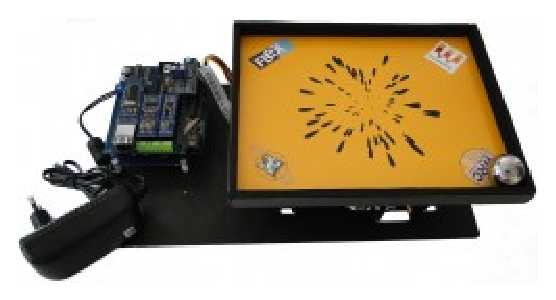
\includegraphics[width=0.6\columnwidth]{ball_and_plate}
  \caption{Ball\&Plate picture.}
  \label{fig:picture}
\end{figure}


\section{Physical model}
\label{sec:model}

In order to present the mathematical model of the ball and plate system,
Figure~\ref{fig:model} shows the $xz$ view of the coordinate system,
introducing the needed parameters to define.
The $yz$ view is identical to the $xz$ view,
considering $\hat{y}$, $y$, $\dot{y}$, $\ddot{y}$, $\theta_y$,
$\omega_y$, $\dot{\omega}_y$ in place of $\hat{x}$, $x$, $\dot{x}$,
$\ddot{x}$, $\theta_x$, $\omega_x$ and $\dot{\omega}_x$, respectively.
Hence, the $yz$ view is omitted.

The sizes of the ball and plate system (in millimeters) are reported in
Table~\ref{tab:measurements}.

Although the real system presents the vertical axes $H$ split in two parts,
as far as we are concerned the proposed model is still valid.
More precisely, the rotation joint is located along the $H$ segment, which means
that it does not coincide with the plate center which in turn is not a fixed
point anymore, causing a greater $\theta$ for the same $alpha$.

A servomotor is in charge of imposing the angle $\alpha$ which,
through the joint $h$, moves the plate of an angle $\theta$.
The forces, which acts on the ball, are the friction and weight forces.

\begin{figure}[htb]
  \centering

  \psfrag{x}[bc]{\small$\hat{x}$}
  \psfrag{z}[bc]{\small$\hat{z}$}
  \psfrag{plate}[bc]{\small$plate$}

  \psfrag{v}[bc]{\small$x, \dot{x}, \ddot{x}$}
  \psfrag{o}[bc]{\small$\theta, \dot{\omega}, \ddot{\omega}$}

  \psfrag{alpha}[bc]{\small$\alpha$}
  \psfrag{tetha}[bc]{\small$\theta$}
  \psfrag{phi}[bc]{\small$\gamma$}

  \psfrag{H}[bc]{\small$H$}
  \psfrag{D}[bc]{\small$D$}
  \psfrag{r}[bc]{\small$r$}
  \psfrag{b}[bc]{\small$b$}
  \psfrag{h}[bc]{\small$h$}
  \psfrag{l}[bc]{\small$l$}
  \psfrag{r}[bc]{\small$r$}
  \psfrag{R}[bc]{\small$R$}

  \psfrag{mg}[bc]{\small$m\overline{g}$}
  \psfrag{F}[bc]{\small$\overline{F}$}
  \psfrag{N}[bc]{\small$\overline{N}$}

  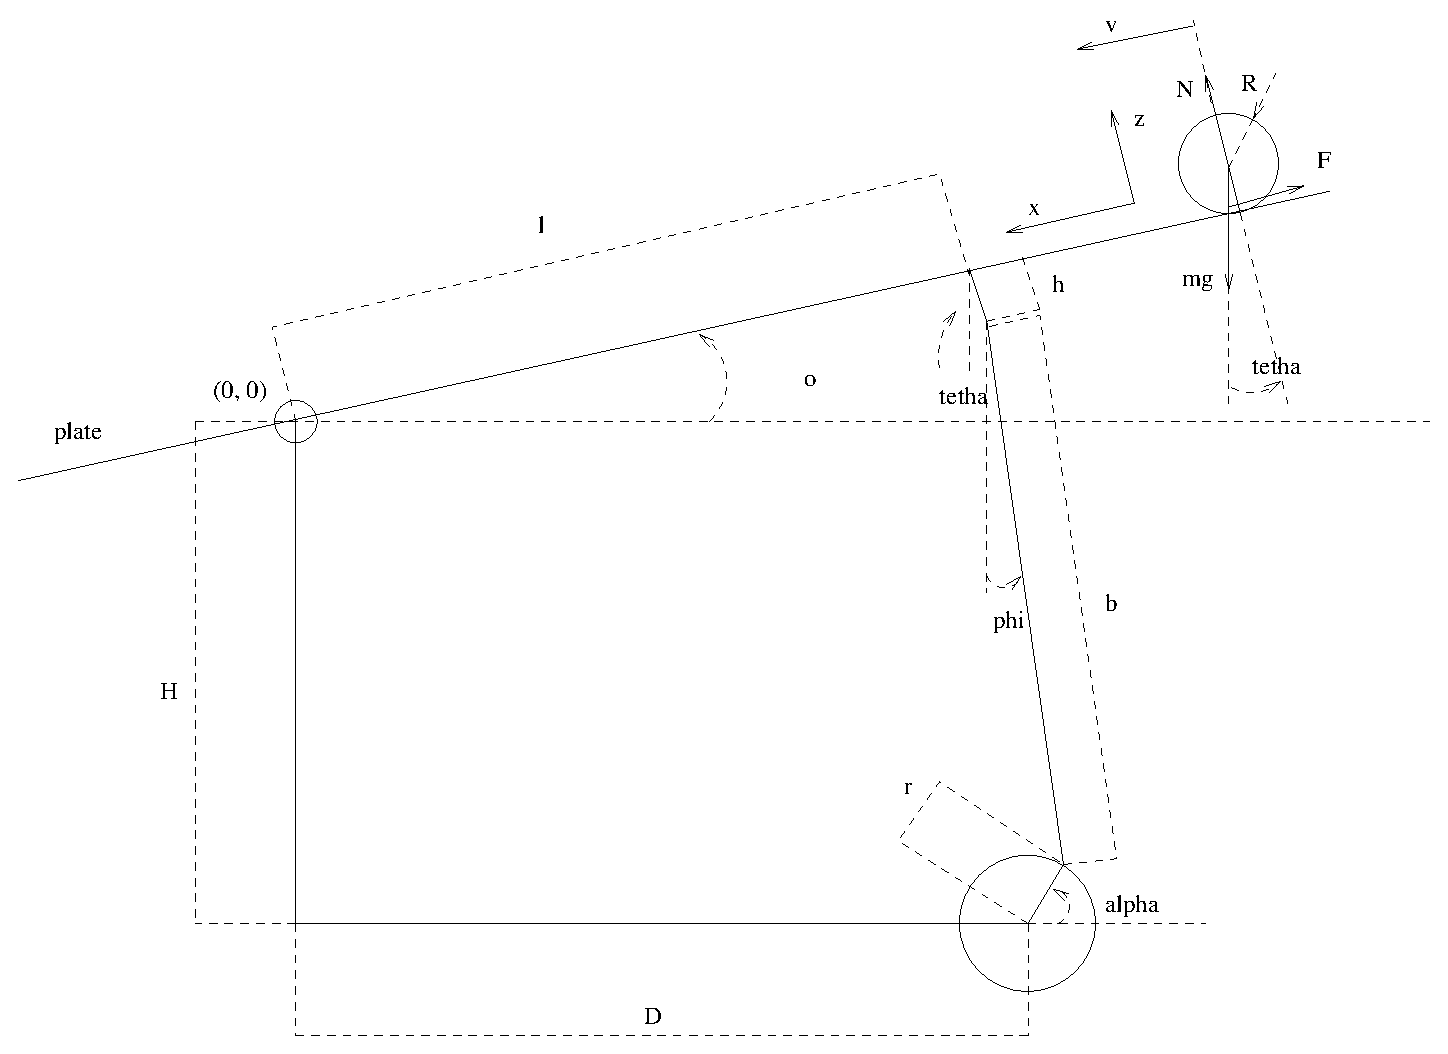
\includegraphics[width=0.9\columnwidth]{model}
  \caption{Physical model.}
  \label{fig:model}
\end{figure}

\begin{table}
	\centering
	\begin{tabular}{ |c|c|c|c|c|c|c|c|c| }
		\hline
		$l_x$ & $l_y$ & $D_x$ & $D_y$ & $H_x$ & $H_y$ & $h$ & $b$ & $r$\\
		\hline
		76    & 62    & 66.5  & 53    & 47    & 49    & 16  & 40  & 20\\
		\hline
	\end{tabular}
	\caption{Plate measurements (mm).}
	\label{tab:measurements}
\end{table}



\section{Mathematical model}
\label{sec:math}

\subsection{Motion laws}
\label{sec:motion}

The complete set of equations is continuous, non-linear and couples the two modes
of motion. After a discretization and linearization process about the operating
point, which is the equilibrium configuration
($x = y = \theta_x = \theta_y = 0$), the equations of motion for the ball,
along the $x$ and $z$ axis, are the following:

\begin{align*}
\ddot{x}[k] &= \frac{5}{7}\ g\ sin (\theta_x[k]) - \left ( r_b + \frac{5}{7}\ h \right ) \dot{\omega}_x[k];\\
%\frac{7}{5} \ddot{y} + \left ( \frac{7}{5} r_b + h \right ) \dot{\omega}_y &= g sin (\theta_y)
m\ddot{z}[k] &= N - mg\ cos(\theta_x[k]) = 0;\\
%\dot{x}[k] &= \frac{ x[k] - x[k-1] } {\Delta t}\\
\dot{x}[k] &= \ddot{x}[k] \Delta t + \dot{x}[k-1];\\
x[k] &= \dot{x}[k] \Delta t + x[k-1];\\
\omega[k] &= \frac{ \theta[k] - \theta[k-1] } {\Delta t};\\
\dot{\omega}[k] &= \frac{ \omega[k] - \omega[k-1] } {\Delta t}.
\label{eq:kinematic}
\end{align*}

Where $\Delta t$ is the updating period (the time elapsed since the previous
check event until the actual). The first two equations are computed
according to the Newton's laws and the last four by the classical kinematic
formulas, assuming a motion uniformly accelerated during each $\Delta t$.

The final kinematic formula to model the ball motion is shown in
Equation~\ref{eq:final_kinematic}.
\begin{equation}
\begin{aligned}
	x[k] &= \ddot{x}[k] \Delta t^2 + \dot{x}[k-1] \Delta t + x[k-1] =\\
		 &= \left[ \frac{5}{7}g \sin(\theta_x[k]) - \left( r_b + \frac{5}{7} h \right) \dot{\omega}_x[k] \right] \Delta t^2 +
			\dot{x}[k-1] \Delta t + x[k-1].
\end{aligned}
\label{eq:final_kinematic}
\end{equation}

\subsection{Angles}
\label{sec:angles}

The relation between $\alpha$ and $\theta$ is given by the closed chain geometry
(considering negligible the elastic coefficient of the plate structure).

\begin{equation}
\left\{
\begin{aligned}
	\hat{x}: & \quad l\ cos(\theta) + h\ sin(\theta) = D + r\ cos(\alpha) + b\ sin(\gamma)\\
	\hat{y}: & \quad H + l\ sin(\theta) = r\ sin (\alpha) + b\ cos(\gamma) + h\ cos(\theta)
\end{aligned}
\right.
\label{eq:basic_model}
\end{equation}

The angle $\gamma$ can be removed and, exploiting the trigonometric axiom
$sin(\beta)^2+cos(\beta)^2=1$, the problem can be rewritten as:

\begin{equation}
[H + l\ sin(\theta) - r\ sin (\alpha) - h\ cos(\theta)]^2 +
[l\ cos(\theta) + h\ sin(\theta) - D - r\ cos(\alpha)]^2 = b^2.
\label{eq:simple_model}
\end{equation}

The relation $\theta = f(\alpha)$ which binds the servomotor angle and the plate
inclination can be better formulated solving Equation~\ref{eq:simple_model}.

\begin{equation}
\begin{aligned}
1: \quad & \{[H + l\ sin(\theta)] - [r\ sin (\alpha) + h\ cos(\theta)]\}^2 + \{[l\ cos(\theta) + h\ sin(\theta)] - [D + r\ cos(\alpha)]\}^2 = b^2;\\
2: \quad & [H + l\ sin(\theta)]^2 + [r\ sin (\alpha) + h\ cos(\theta)]^2 - 2 [H + l\ sin(\theta)][r\ sin (\alpha) + h\ cos(\theta)] +\\
   & + [l\ cos(\theta) + h\ sin(\theta)]^2 + [D + r\ cos(\alpha)]^2 - 2 [l\ cos(\theta) + h\ sin(\theta)] [D + r\ cos(\alpha)]= b^2;\\
3: \quad & H^2 + l^2 sin(\theta)^2 + 2 H l sin(\theta) + r^2 sin (\alpha)^2 + h^2 cos(\theta)^2 + 2 r h sin (\alpha) cos(\theta) +\\
   & - 2 H r sin (\alpha) -2 l r sin(\theta) sin(\alpha) -2 H h cos(\theta) -2 l h sin(\theta) cos(\theta) +\\
   & + l^2 cos(\theta)^2 + h^2 sin(\theta)^2 + 2 l h cos(\theta) sin(\theta) + D^2 + r^2 cos(\alpha)^2 + 2 D r cos(\alpha) +\\
   & - 2 l D cos(\theta) - 2 l r cos(\theta) cos(\alpha) - 2 h D sin(\theta) -2 h r sin(\theta) cos(\alpha)= b^2;\\
4: \quad & b^2 = H^2 + l^2 + r^2  + h^2 + D^2 + 2 D r cos(\alpha) - 2 H r sin(\alpha) +\\
   & + 2 cos(\theta) [ h r sin(\alpha) - H h - l D - l r cos(\alpha) ] + 2 sin (\theta) [ H l - l r sin(\alpha) - h D - r h cos(\alpha)].
\end{aligned}
\label{eq:f_alpha}
\end{equation}

In order to make the model easier, it is linearized considering small swings of
$\theta$ which means that $sin(\theta)=\theta$ and $cos(\theta)=1$.
From this perspective, the result of Equation~\ref{eq:f_alpha} can be rewritten
as reported in Equation~\ref{eq:f_alpha_small_swings}.

\begin{equation}
\begin{aligned}
& b^2 = H^2 + l^2 + r^2  + h^2 + D^2 + 2 D r cos(\alpha) - 2 H r sin(\alpha) +\\
& + 2 [ h r sin(\alpha) - H h - l D - l r cos(\alpha) ] + 2 \theta [ H l - l r sin(\alpha) - h D - r h cos(\alpha)].
\end{aligned}
\label{eq:f_alpha_small_swings}
\end{equation}

Expressing the formula in function of $\theta$ will lead to
Equation~\ref{eq:theta}.

\begin{equation}
\theta = \frac{H^2 + l^2 + r^2  + h^2 + D^2 + 2 D r cos(\alpha) - 2 H r sin(\alpha) - b^2 + 2 [ h r sin(\alpha) - H h -
l D - l r cos(\alpha) ]}{2 [ l r sin(\alpha) + h D + r h cos(\alpha) - H l]}.
\label{eq:theta}
\end{equation}

Although the plate is in a rest position ($\theta=0^{\circ}$) when the 
servomotor is ordered to hold $0^{\circ}$, the actual $\alpha$ is not
$0^{\circ}$ according to how the ball and plate models have been designed.

$\alpha_{x0}$ and $\alpha_{y0}$ are computed, imposing $\theta=0^{\circ}$ as
shown in Equation~\ref{eq:equilibrium}.
\begin{equation}
\left\{
\begin{aligned}
	\hat{x}: & \quad [H - r\ sin (\alpha_{x0}) - h]^2 + [l - D - r\ cos(\alpha_{x0})]^2 = b^2\\
	\hat{y}: & \quad [H - r\ sin (\alpha_{y0}) - h]^2 + [l - D - r\ cos(\alpha_{y0})]^2 = b^2
\end{aligned}
\right.
\label{eq:equilibrium}
\end{equation}

For the sake of simplicity, the calculus refers only to $x$ axes and it is
reporter in Equation~\ref{eq:equilibrium_1}
\begin{equation}
\left\{
\begin{aligned}
&	A \sin(\alpha) + B \cos(\alpha) + C = 0\\
&	A = 2rh-2Hr\\
&	B = 2Dr-2lr\\
&	C = H^2+r^2+h^2+l^2+D^2-b^2-2Hh-2lD
\end{aligned}
\right.
\label{eq:equilibrium_1}
\end{equation}

In order to solve the trigonometric equation imposing $t=\tan(\frac{x}{2})$
lets us transform the problem into a second order equation, as shown in
Equation~\ref{eq:equilibrium_2}.

\begin{equation}
\left\{
\begin{aligned}
&	t=\tan(\frac{x}{2})\\
&	(C-B)\ t^2 + 2A\ t + B + C = 0
\end{aligned}
\right.
\label{eq:equilibrium_2}
\end{equation}

According to the model parameters defined in Table~\ref{tab:measurements},
the equilibrium angles are $\alpha_{x0}\simeq-38.814^{\circ}$ ($-0.68$ rad) and
$\alpha_{y0}\simeq-30^{\circ}$ ($-0.52$ rad).

For this reason, $\alpha$ needs to be consider as the sum between the rest angle
and the desired angle: $\alpha = \alpha_0 + \alpha'$.

Considering small swings for $alpha$ and the addition formulas\footnotemark,
 trigonometric operations in Equation~\ref{eq:theta} are rewritten as:
\begin{equation}
\begin{aligned}
sin(\alpha) =& \alpha' cos(\alpha_0) + sin(\alpha_0);\\
cos(\alpha) =& cos(\alpha_0) - \alpha' sin(\alpha_0).
\end{aligned}
\label{eq:new_theta}
\end{equation}

\footnotetext[1]{
Addition formulas:
\begin{itemize}
    \item $\sin(\alpha + \beta) = \sin(\alpha) \cos(\beta) + \cos(\alpha) \sin(\beta)$;
    \item $\cos(\alpha + \beta) = \cos(\alpha)\cos(\beta) - \sin(\alpha)\sin(\beta)$.
\end{itemize}
}

The plot of the function $\theta = f(\alpha)$ is depicted in
Figure~\ref{fig:f_alpha} (with $\alpha \in [0, \pi]$), where in $\alpha=2.25$ a
vertical asymptote occurs.

\begin{figure}[htb]
  \centering

  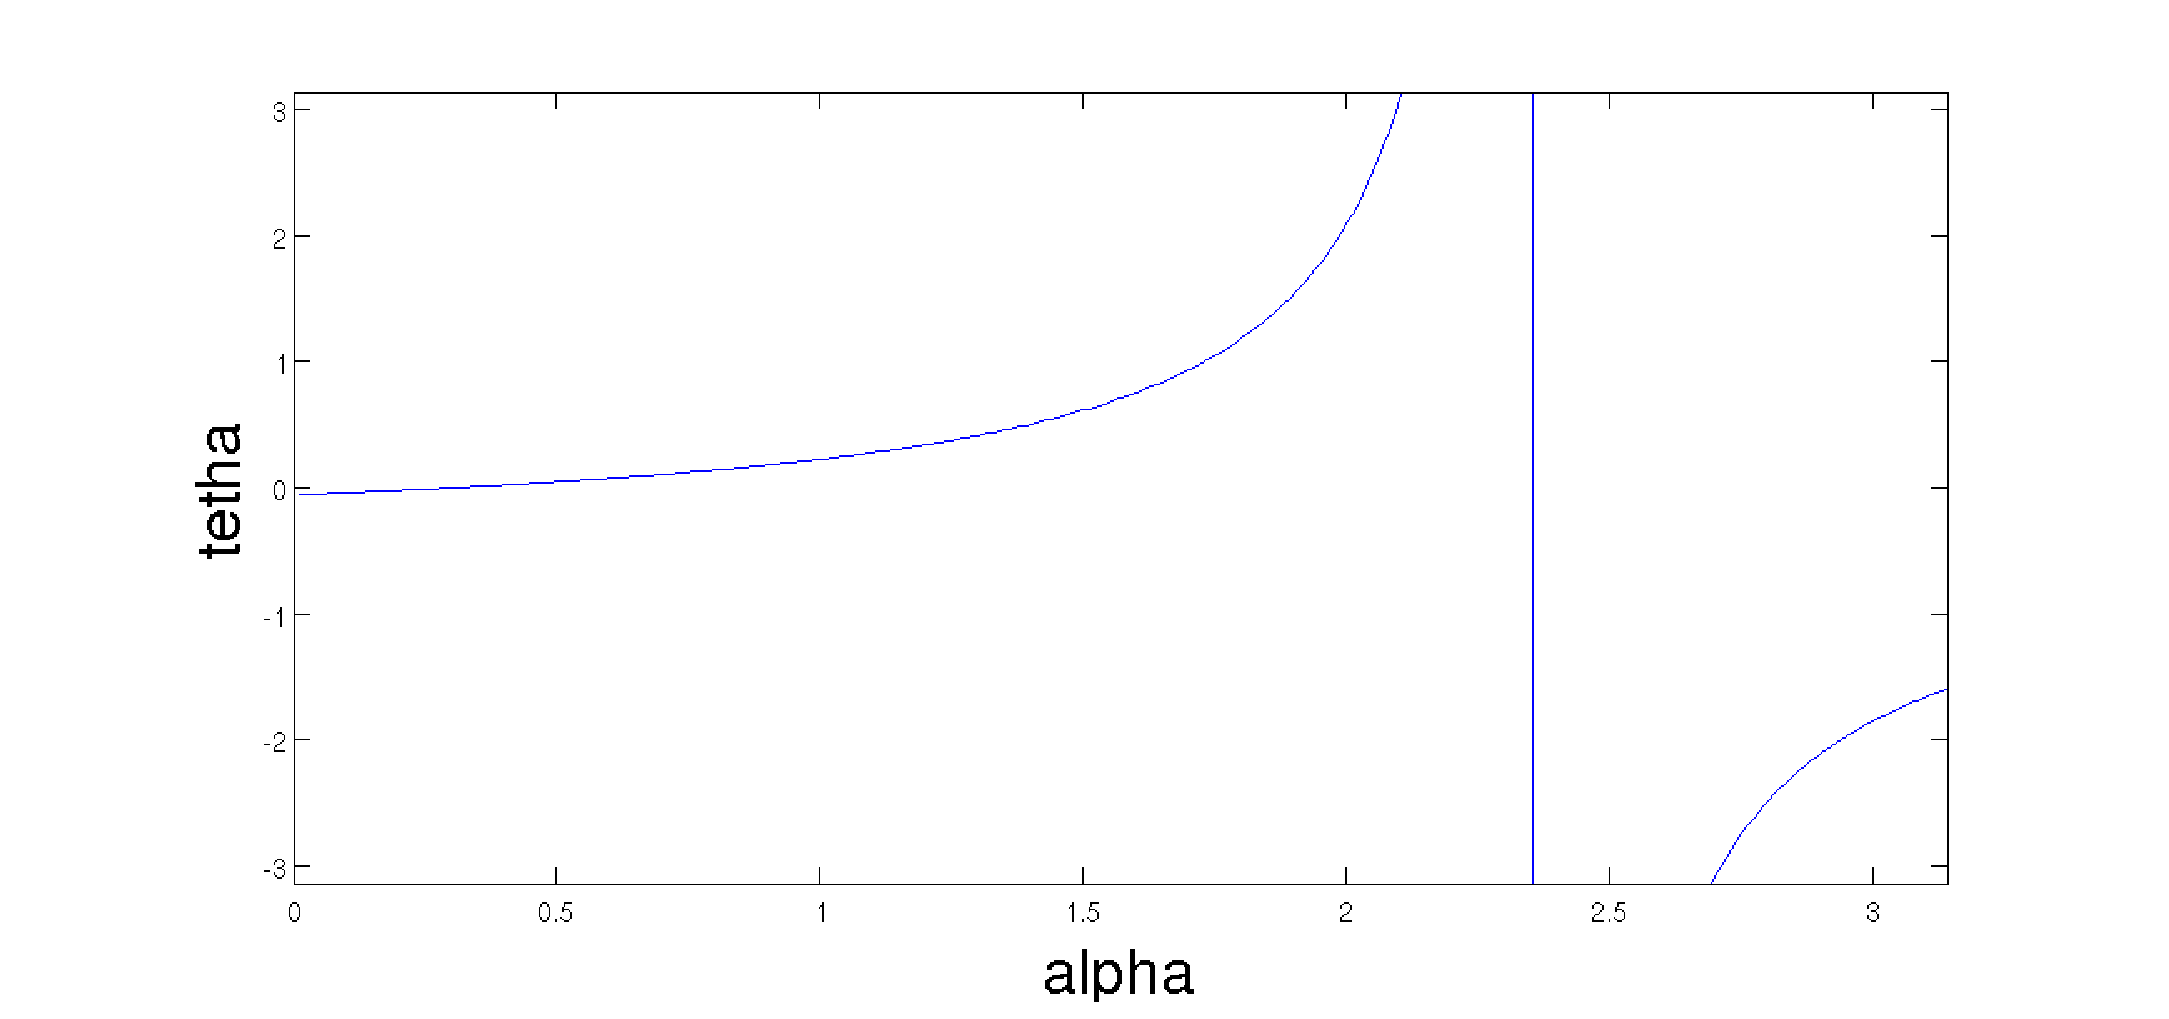
\includegraphics[width=1\columnwidth]{f_alpha}
  \caption{$\theta = f(\alpha)$.}
  \label{fig:f_alpha}
\end{figure}
 


\input{control}


% conference papers do not normally have an appendix




% trigger a \newpage just before the given reference
% number - used to balance the columns on the last page
% adjust value as needed - may need to be readjusted if
% the document is modified later
%\IEEEtriggeratref{8}
% The "triggered" command can be changed if desired:
%\IEEEtriggercmd{\enlargethispage{-5in}}

\bibliographystyle{./styles/IEEEtran}
\bibliography{paper}

\end{document}

